\section{Durchführung}
\label{sec:Durchführung}

\subsection{Bestimmung der Zeitkonstanten}
    Zur Bestimmung der Zeitkonstanten wird der Versuchsaufbau von Abbildung \ref{fig:schalt2} verwendet.
    \begin{figure}
        \centering
        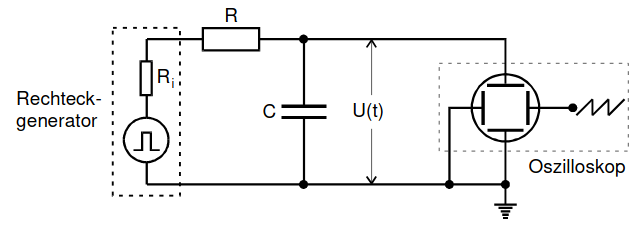
\includegraphics{schalt2.png}
        \caption{Schaltkreis zur Bestimmung der Zeitkonstanten}
        \label{fig:schalt2}
      \end{figure}
    Mit einer Rechteckfrequenz werden periodisch Auf- und Entladevorgänge des Kondensators 
    generiert. Mittels eines Oszilloskops wird die Spannung am Kondensator über mehrere
    Auf- und Entladevorgänge gemessen. Mit Hilfe dieser Daten kann dann anhand der in der 
    Theorie hergeleiteten Formeln die Zeitkonstante $RC$ bestimmt werden. 

\subsection{Bestimmung der Frequenzabhängigkeit der Kondensatoramplitude}
    \begin{figure}
        \centering
        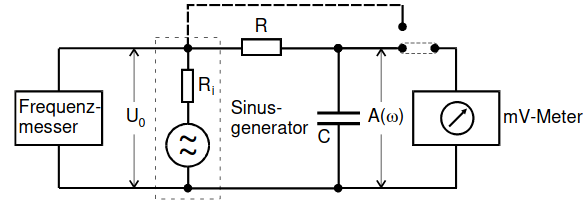
\includegraphics{schalt4.png}
        \caption{Schaltkreis zur Untersuchung der Frequenzabhängigkeit der Kondensatorspannung}
        \label{fig:schalt4}
    \end{figure}
    Für diesen Versuchsteil wird der Stromkreis von Abbildung \ref{fig:schalt4} verwendet. Es wird
    eine Sinusspannung angelegt und die Kondensatorspannung in Abhängigkeit der angelegten
    Frequenz bestimmt. Die Kondensatorspannung wird nun unter Zuhilfenahme eines 
    Millivoltmeters gemessen.

\subsection{Bestimmung der Phasenverschiebung}
    Nun wird sowohl die angelegte Sinusspannung als auch die Kondensatorspannung mit einem
    Oszilloskop aufgezeichnet, so wie in Abbildung \ref{fig:schalt1} dargestellt. 
    \begin{figure}
        \centering
        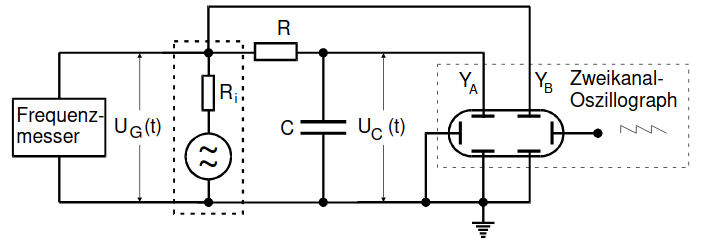
\includegraphics{schalt1.png}
        \caption{Schaltkreis zur Messung der Phasenverschiebung}
        \label{fig:schalt1}
    \end{figure}
    Dadurch entsteht ein 
    Schirmbild gleich jenem in Abbildung \ref{fig:sinus} . 
    \begin{figure}
        \centering
        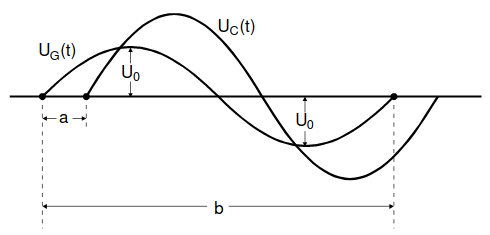
\includegraphics{sinus.png}
        \caption{theoretisches Schirmbild des Oszilloskops}
        \label{fig:sinus}
    \end{figure}
    Die Phase kann dann durch $\phi = \dfrac{a}{b} 2\pi$
    berechnet werden, wobei a den zeitlichen Abstand der Nulldurchgänge und b der Periodendauer
    entspricht.

\subsection{Der RC-Kreis als Integrator}
    Für diesen Aufgabenteil kann erneut Schaltkreis ... verwendet werden. Nachdem  eine geeignete
    Frequenz ausgewählt wurde kann die Kondensatorspannung bei Rechteck-, Sinus- und Dreiecksspannung
    bestimmt werden.